\section{Snow Simulator}

The snow simulator has been developed over several years by different students in 
the HPC-lab at NTNU. It simulates a finite number of snow particles and how they 
are affected by the wind and terrain. 

\subsection{History}

The snow simulator was originally developed  by Ingar Saltvik for his master
thesis \emph{"Parallel Methods for Real-Time  Visualization of Snow"}
\cite{originalSnowThesis}. Saltvik's implementation was  designed for multi-core
CPUs and achieved real-time performance for tens of  thousands snow particles
and unknowns for the wind simulation.

TODO: Insert figure of Saltvik's snow simulator

The snow simulator was later ported to the GPU by Robin Eidissen for his master 
thesis \emph{"Utilizing GPUs for Real-Time Visualization of Snow"}\cite{gpuSnowThesis}.
Eidissen's implementation achieved real-time performance with more than two million 
snow particles and four million unknowns in the wind simulation. 

TODO: Insert figure of the GPU snow simulator

TODO: Write about the other master theses and specialization projects that 
have worked on the snow simulator

%The following master theses have done work on the snow simulator:
%
%\begin{itemize}
%	\item Enhancing and Porting the HPC-Lab Snow Simulator to OpenCL on Mobile Platforms
%	\cite{openclSnowThesis}
%	\item Terrain Rendering Techniques for the HPC-Lab Snow Simulator\cite{snowTerrainThesis}
%	\item Enhancing the HPC-Lab Snow Simulator with More Realistic Terrains and Other Interactive Features
%	\cite{realisticSnowTerrainThesis}
%	\item Ray Tracing for Simulation of Wireless Networks in 3D Scenes\cite{rayTracingThesis}
%	\item OpenACC-based Snow Simulation\cite{openAccThesis}
%	\item Avalanche Simulations using Fracture Mechanics on the GPU\cite{avalancheThesis}
%\end{itemize}

\subsection{Overview}

The snow simulator is written in a combination of C, C++ and CUDA.
The four main components of the snow simulator is the \emph{wind simulator}, 
\emph{snow simulator}, \emph{terrain} and the \emph{renderer}. The wind and 
snow simulators are written CUDA and compiled separately using the NVCC compiler 
into a external library called \emph{particle}. The wind simulator 
solves the incompressible Euler equations to calculate the wind velocity field. 
The wind simulator uses the terrain to create obstacles for the wind. The snow 
simulator uses the result from the wind simulator to update the position of the 
snow particles. When a snow particle lands on the ground it is added to the terrain.
The terrain uses a heightmap to identify the snow buildup.

\begin{figure}[ht]
	\center
	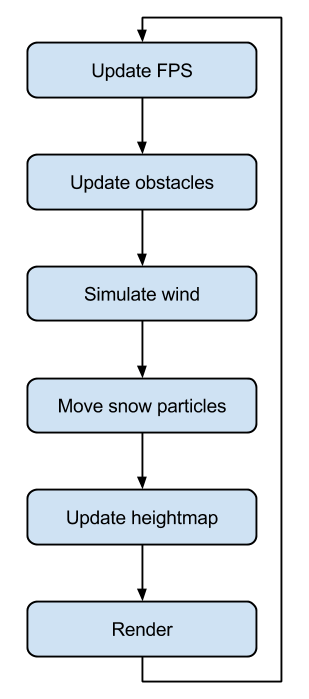
\includegraphics[width=0.30\textwidth]{images/snow_sim_main_loop}
	\caption{Snow simulator main loop.}
	\label{fig:mainLoop}
\end{figure}

\subsection{Wind Simulation}

The wind simulation calculates the three dimensional wind velocity field through
computational fluid dynamics (CFD). The discretization method being used is the
finite difference method. The boundary conditions for the CFD problem is decided
by the terrain vertex data and the external wind velocity at the borders of the
domain. The external wind velocity can be set by the user at runtime. The system
is solved using a SOR- solver and the boundary conditions are satisfied by
adjusting cells that are next to obstacles.

\subsubsection{Implementation}

The wind simulator is implemented in CUDA and consists of eight kernels. Five of 
the kernels are used for simulation while the remaining three kernels are for 
visualization. The wind simulation uses the following data structures:

\begin{description}
	\item[wind\_vel,] a three dimensional array of float4 representing the wind 
	velocity field. At the end of the wind simulation step, the contents of this 
	array is moved to texture memory for efficient access by the snow particle 
	simulation. 
	\item[obstacle,] a three dimensional array of integers. The bits of each 
	integer indicate if the current cell or an neighboring cell contains an 
	obstacle. 
	\item[pressure,] a three dimensional array of floats containing the values 
	of the air pressure used in the projection step of the wind simulator. 
	\item[solution,] a three dimensional array of floats containing the solution 
	vector (right-hand side) for the Poisson equation. 
\end{description}

Each of the five simulation kernels handles a part of solving the momentum equation 
of the incompressible Euler equations.
\begin{description}
	\item[wind\_advect]
	\item[build\_solution2]
	\item[solve\_poisson2]
	\item[set\_boundary2]
	\item[wind\_project2]
\end{description}

The visualization kernels are used to visualize the data structures used when 
simulating the wind. These are the visualization kernels:

\begin{description}
	\item[make\_obs\_points,] visualizes the cells determined to be obstacles 
	for the wind from the terrain. 
	\item[make\_pressure\_points] colormapped points to visualizes the pressure 
	in the cells. 
	\item[make\_vel\_lines] visualizes the wind velocity field as field lines 
	colormapped depending on the magnitude of the wind velocity vector. 
\end{description}

